A problem in finding and tracking a particle was that the surface of the PDMS was very uneven and sharp ridges along the length of the channel appear as in figure \ref{fig:unpolished} unless the focus was in a relatively narrow depth of the channel. 
 
 \begin{figure}[H]
 \centering
 \begin{subfigure}[3a]{0.40\textwidth}
 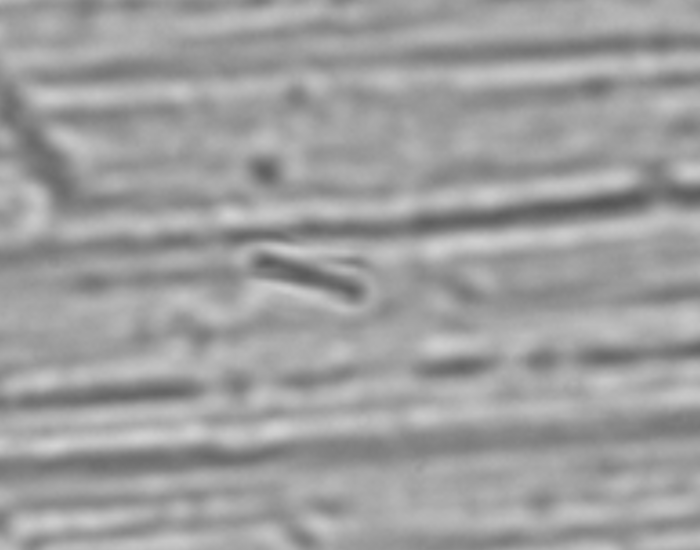
\includegraphics[width=\textwidth]{figures/improvements/unpolished.png}
 \caption{An unusually severe case of the PDMS edges creating noise.}\label{fig:unpolished}
 \end{subfigure}\hspace{1em}%
 \begin{subfigure}[3b]{0.40\textwidth}
 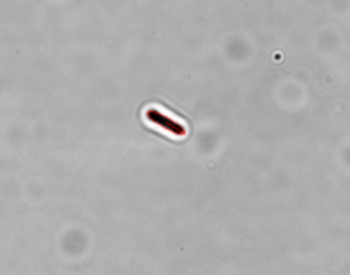
\includegraphics[width=\textwidth]{figures/improvements/polished.png}
 \caption{After being polished there is no trace of such ridges.}\label{fig:polished}
 \end{subfigure}
 \caption{Pictures highlighting the roundness of the particles as well as the apparent symmetry of some particles. It should be noted that although there are no apparent rough edges there was no way to rotate a sample so there might very well be asymmetries on the side of the particle that we cannot see.}
 \label{fig:polisheffect}
 \end{figure}
 

This was fixed by polishing the copper mold in which the PDMS channels are formed with a silicate abbrasive (Autosol) and emery cloth. This was shown to remove all visible scratches from the mold and thus from the PDMS. As seen in Figure \ref{fig:polished} no scratches can be detected.